\documentclass[a4paper, 11pt]{exam}
\usepackage{titling}
\newcommand{\subtitle}[1]{%
  \posttitle{%
    \par\end{center}
    \begin{center}\large#1\end{center}
    }%
}

\usepackage{url}
\usepackage{amsmath,amsthm,enumitem,amssymb}
\usepackage{graphicx}
\usepackage{hyperref}
\usepackage{float}
\renewcommand{\labelenumii}{\roman{enumii}}

\title{Homework Assignment 5}
\subtitle{CS/ECE 6810: Computer Architecture \\
Apr 10,2018\\
Marek Baranowski}

\begin{document}
\maketitle
\begin{enumerate}
\item Virtually Indexed Caches

From 
\begin{verbatim}
https://www.ece.cmu.edu/~ece447/s12/lib/exe/fetch.php?media=wiki:18447-l21.pdf
\end{verbatim}
we see that if the L1 cache is sized such that 
$cache\_entries\le(page\_size\cdot associativity)$ then a if page offset is smaller
than the Index and Offset, then the CPU will be able to access each cache
entry uniquely, so we can keep the simple, concurrent TLB/cache look up scheme
we saw in class.

If on the other hand we have $cache\_entries>(page\_size\cdot associativity)$
then the cache index will need to take some of the lower bits from the VA to
index the cache. This leads to a ``synonym'' problem where two VAs that map
to contiguous PAs appear to map to different sets in the cache. This is 
undesirable since we will have two cache lines occupied for the same memory,
leading to an incoherent view of memory. This type of indexing is referred to
as ``virtually indexed, physically tagged'' as part of the VA is used. There 
areways around the synonym situation:

A very simple solution is mentioned in:
\begin{verbatim}http://www.youtube.com/watch?v=cP3zeaDcq6A\end{verbatim}
where we perform the TLB lookup {\em before} indexing into the cache, this
provides the necessary lower PA bits to correctly index the cache. Obviously
this is undesirable as we have a longer critical path when accessing the cache.

The first reference mentions the method for handling this situation on
the Alpha 21264 and MIPS R10K, which when a write occurs, all possible matches
are considered and once the result from the TLB is known, invalidation and
update can occur.


Another solution mentioned in the two prior references is to use ``page
coloring''. In this scheme, the OS ensures VAs that should map to the same 
cache entry each have the same lower order bits so they match the PA, allowing 
the TLB lookup to be done concurrently with the cache lookup. 

From ``Page Placement Algorithms for Large Real-Indexed Caches'' by Kessler and
Hill, there are some disadvantages to this simple scheme: inter-process VAs
will tend have contention over the same cache set, to alleviate this the authors
propose a scheme where the processes PID is hashed with the VA index bits. This
tends to make contention unlikely for frequently accesses memory locations, like
the stack (which is placed at the same VA for all processes without address
layout randomization). This scheme is also weak when memory is low as the 
address assignment algorithm will be forced to choose a physical page with a
non-matching address.

Kessler and Hill discuss three other methods, each with strengths and 
weaknesses, they are:
\begin{enumerate}
\item Bin Hopping
\item Best Bin
\item Hierarchical mapping
\end{enumerate}

\item Cache and Memory Model using CACTI

\begin{enumerate}
\item For both caches I used the ``itrs-hp'' data cell type. The L1 cache
was set to ``fast'' data access and for the L2 cache I used ``normal'' data
access. L1 has 17 tag bits, and L2 has 14 tag bits (which were calculated
in assignment 4, except we had a 33-bit address space). Both use 128 bit data
buses.

For the L1 cache we have the following properties from CACTI:
\begin{verbatim}
Cache Parameters:
    Total cache size (bytes): 32768
    Number of banks: 1
    Associativity: direct mapped
    Block size (bytes): 16
    Read/write Ports: 1
    Read ports: 0
    Write ports: 0
    Technology size (nm): 32

    Access time (ns): 0.345662
    Cycle time (ns):  0.446902
    Total dynamic read energy per access (nJ): 0.0136127
    Total leakage power of a bank (mW): 12.4047
    Cache height x width (mm): 0.164353 x 0.469618 = .0772 mm^2
    Data array space efficiency: 59.6743%
    Tag array space efficiency: 67.1195%
\end{verbatim}
And for L2 we have these properties:
\begin{verbatim}
Cache Parameters:
    Total cache size (bytes): 1048576
    Number of banks: 1
    Associativity: 4
    Block size (bytes): 64
    Read/write Ports: 1
    Read ports: 0
    Write ports: 0
    Technology size (nm): 32

    Access time (ns): 1.07383
    Cycle time (ns):  1.34504
    Total dynamic read energy per access (nJ): 0.241674
    Total leakage power of a bank (mW): 327.818
    Cache height x width (mm): 1.06087 x 1.77384 = 1.882 mm^2
    Data array space efficiency: 75.1545%
    Tag array space efficiency: 76.0056%
\end{verbatim}
There are a few things to note here: L2 access times are about 3 times slower
than L1 access times. But this comes at a somewhat significant cost where the
L2 cache is using about 26 times more energy than the L1 cache. However, this is
to be expected as the L2 needs at a minimum 32 times the number of
transistors that L1 requires due to their differing sizes. This result actually
implies the L2 cache is slightly more efficient with leakage power per stored
bit than the L1 cache.

The dimensions of both caches are notable: L1 is about 4 times as wide
as it is tall, whereas L2 has a ratio between height and width of
about 1.5.  Playing with the parameters of each cache, this disparity
is due to the L1 cache's small size along with its being direct mapped
and size of its cache line. Interestingly only changing the L1 cache
size and associativity leads to a configuration with the same space
efficiencies. As reported by CACTI, the L1 cache is about 10\% less
space efficent than L2. We can see this in the ratio of the areas of
the cache sizes with L2 being about 24 times larger than L1, but L2 is
storing 32 times as much information. From
$\frac{28}{32}\approx87.5\%$ we can see directly the inefficiency of
the L1 cache in terms of its area; the L2 cache is using 0.75 times the area per
bit.
\item Below are the plots for access time, access energy, leakage power and area
for differing amounts of associativity for the L2 cache.
\begin{figure}[H]
\begin{centering}
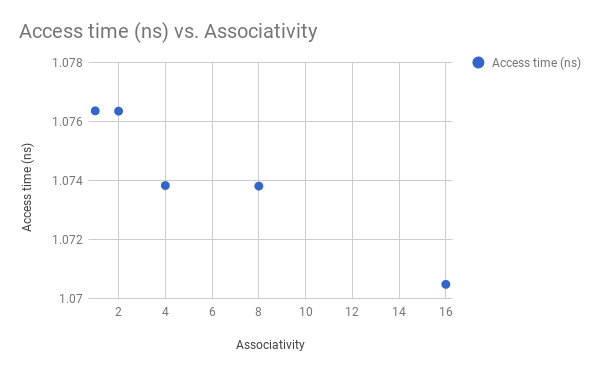
\includegraphics[width=.5\linewidth]{AccessTime.png}
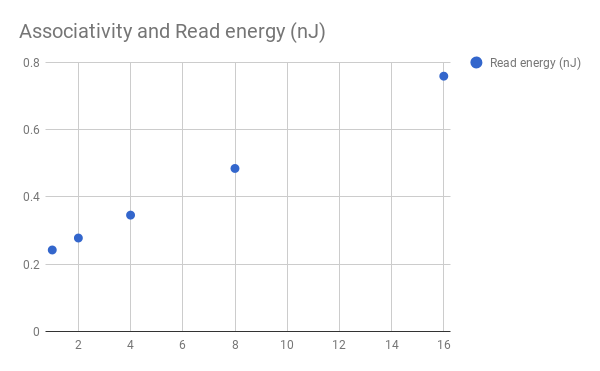
\includegraphics[width=.5\linewidth]{Energy.png}
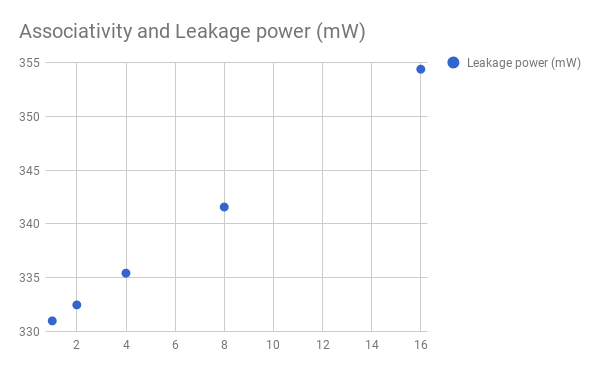
\includegraphics[width=.5\linewidth]{Leakage.png}
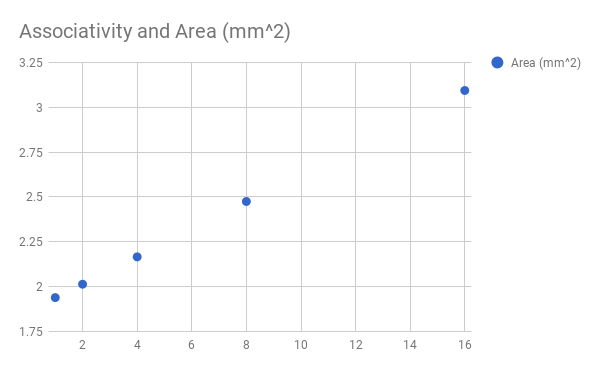
\includegraphics[width=.5\linewidth]{Area.png}
\end{centering}
\end{figure}
It is very clear from comparing these plots that we meet diminishing
returns very quickly by increasing associativity. When associativity
is 16, the L2 cache is about .005ns faster than when accosiativity is
1. It becomes very apparent at 16 that the energy, leakage and areas
are increasing faster than linearly (these circuits have capacitance),
and we are not getting much in return from access times. It appears
from the graphs that 4 way associativity may be the best trade off
between access time and area, energy and power: 8 way associativity
uses about 40\% more energy per access, leaks 6 more mW and occupies
14\% more die space while having only slightly better access times
than 4 way associativity. But in reality, the ideal cache parameters
would be determined by the application.

The increases in energy, leakage power and die area are to be expected since
the higher associativity requires more circuitry to select the correct portion
of the cache entry.

\end{enumerate}
\end{enumerate}


\end{document}